\pagebreak
\subsection{Thermal Design} \label{Thermal_section}

\subsubsection{Thermal Environment}
\begin{centering}
The experiment experienced a wide temperature range during the flight and it was able to continue operating despite these changes due to the incorporated thermal design. As seen in Figure \ref{fig:temperature-profile}, the coldest point of the flight was between 10 km and 15 km where the air temperature can drop to $-70\degree{C}$ outside. During the flight the coldest recorded temperature on the gondola was $-54\degree{C}$ during the Ascent and Descent.
% Phases\cite{BexusManual}. %Sampling with the AAC were planned to begin when the balloon had risen to 18 km during the Ascent Phase and will last until the Float Phase but since there were a failure no sampling were done . Sampling will resume when the gondola has fallen to 17.5 km during the Descent Phase. This means the experiment will be above the coldest part of the atmosphere and the critical components will have time to achieve their operating temperature before sampling time commences. 
In addition, launching from Kiruna in late October meant the temperature on the ground could be as low as $-10\degree{C}$ but the temperature at the time for launch ended up being around $0\degree{C}$. 
As the component with the warmest lower limit operating temperature had to be kept at a minimum of $5\degree{C}$ (E3 in Table\ref{tab:thermal-table}), this  required the heaters to be switched on while the experiment was still on the ground.
\end{centering}

\begin{figure}[H]
    \begin{align*}
        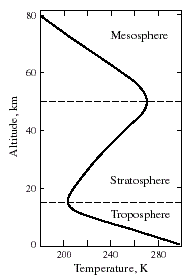
\includegraphics[height=8cm]{4-experiment-design/img/temperature-profile.png}
    \end{align*}
    \caption{Diagram Showing the Temperature Profile of the Atmosphere \cite{jacob}.}\label{fig:temperature-profile}
\end{figure}

\subsubsection{The Critical Stages}
The flight had the following critical stages:
\begin{itemize}
    \item Launch pad
    \item Early ascent
    \item Sampling ascent
    \item Float
    \item Descent before sampling
    \item Sampling descent
    \item Shut down
    \item Landed, waiting for recovery
\end{itemize}
These stages were accounted for in further calculations and simulations.

\subsubsection{Overall Design}
To protect the components against the cold, a thermal control system was designed. Insulation and internal heating both came into play in keeping all the components functional throughout the duration of the flight. The two components with the most critical thermal ranges were the pump and the valve manifold system (E3 and E5 in Table \ref{tab:thermal-table}). Thermal regulation elements were designed with the main focus having been on the AAC, however a thermal analysis of the CAC can be found in Appendix \ref{sec:appI} under Section \ref{sssec:CAC-trial-flight} where in the CAC box the valve was identified as the critical component in terms of thermal regulation (refer to component E5 in Table \ref{tab:thermal-table}). It had a current through it throughout the flight, therefore heating it self up.

% New for the SED v2
The main protection against the cold environment in the stratosphere was a passive thermal design by means of insulating layers added to the walls of the experiment. It was comprised of two layers: one outer sheet of aluminum and a thicker sheet of Styrofoam. The main insulating factor was Styrofoam, which significantly reduced the heat exchange between the otherwise exposed experiment box, and also provided shock absorption when the gondola landed after separating from the balloon.

\begin{figure}[H]
    \centering
    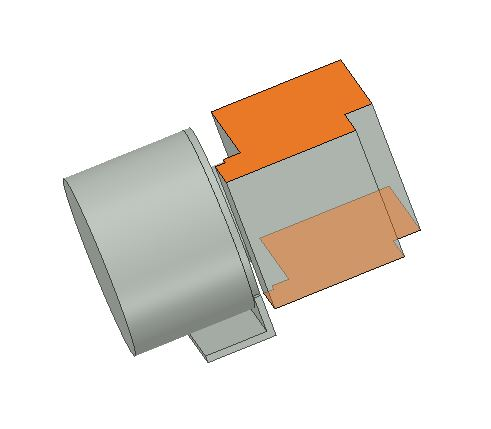
\includegraphics[width=0.5\linewidth]{4-experiment-design/img/Thermal/higlighted-heater-pump.JPG}
    \caption{Highlight of the Heater On the Pump.}
    \label{fig:highlight-heater-on-pump}
\end{figure}

An active thermal control system consisting of four heaters was also implemented. Two heaters were placed as seen in Figure \ref{fig:highlight-heater-on-pump} and a single heater was placed on the flushing valve temperature and one heater was placed on the manifold. To control these heaters, two temperature sensors were also on board, one attached to the pump and the other attached to the manifold. If the reading from one of the temperature sensors was lower than the predefined threshold, then the heater turned on and warmed the component. If it was above the higher threshold the heater turned off.

Simulations in MATLAB (code can be found in Appendix \ref{sec:appJ}) were used to determine the average uniform heat inside the experiment. The ANSYS thermal modelling platform was used to the simulate the thermal conditions inside the Brain.

Table {\ref{tab:thermal-table-4}}, below, covers the thermal ranges of the components crucial to the experiment flight from those listed in Section \ref{sec:experiment-components}:



%Added this space to help us see all of the numbers. This "Track changes" sign blocks them every time!


\begin{longtable}{|m{1cm}|m{3.5cm}|m{1.3cm}|m{1.3cm}|m{1.4cm}|m{1.3cm}|m{1.3cm}|m{1.3cm}|}
\hline
\multirow{2}{*}{\textbf{ID}} & \multirow{2}{*}{\textbf{Components}}                                 & \multicolumn{2}{l|}{\textbf{Operating (°C)}} & \multicolumn{2}{l|}{\textbf{Survivable (°C)}} & \multicolumn{2}{l|}{\textbf{Expected (°C)}} \\ \cline{3-8} &   & Min.  & Max.  & Min.  & Max.  &  Min.   &  Max.            \\ \hline
E1 & Arduino Due & -40 & 85 & -60 & 150 & -15.7 & 54.0 \\ \hline
E2 & Ethernet Shield & -40 & 85 & -65 & 150 & -15.7 & 54.0 \\ \hline
E3 & Miniature diaphragm air pump & 5 & 40 & -10 & 40 & 10 & 34.9 \\ \hline
E4 & Pressure Sensor & -40 & 85 & -40 & 125 & -15.7 & 54.0 \\ \hline
E5 & Sampling Valve (inlet and outlet 1/8"" female) & -20 & 68 & -20\footnote{If survivable temperatures were not given, operating temperatures were used as survivable limits.\label{fn:erik}} & 68\textsuperscript{\ref{fn:erik}} & -15 & 20 \\ \hline
E6 & Airflow sensor AWM43300V & -20 & 70 & -20\textsuperscript{\ref{fn:erik}} & 70\textsuperscript{\ref{fn:erik}} & -8.8 & 34.9 \\ \hline
E7 & Heater ($12.7\times 50.8 mm$) & -200 & 200 & -200\textsuperscript{\ref{fn:erik}} & 200\textsuperscript{\ref{fn:erik}} & -20 & 36 \\ \hline
%E8 & Voltage Regulator & -40 & 125 & -40\textsuperscript{\ref{fn:erik}} & 125\textsuperscript{\ref{fn:erik}} & -30.62 & 34.93 \\ \hline
E9 & Temperature Sensor & -55 & 125 & -65 & 150 & -19.7 & 43 \\ \hline
E10 & DCDC 24 V & -40 & 85 & -55 & 125 & -15.7 & 54.0 \\ \hline
E12 & Micro SD & -25 & 85 & -200\textsuperscript{\ref{fn:erik}} & 200\textsuperscript{\ref{fn:erik}} & -15.7 & 54.0 \\ \hline
%E13 & Logic CAT5E & -55 & 60 & -55\textsuperscript{\ref{fn:erik}} & 60\textsuperscript{\ref{fn:erik}} & -34 & 15 \\ \hline
% E14 & Resistors (33, 150 and 100 ohm) & -55 & 155 & (-55)\textsuperscript{\ref{fn:erik}} & (155)\textsuperscript{\ref{fn:erik}} & TBD\textsuperscript{\ref{fn:ivan}} & TBD\textsuperscript{\ref{fn:ivan}} \\ \hline
% E15 & Capacitors $(0.1 \mu$ F and $10 \mu$ F) & -30 & 85 & (-200)\textsuperscript{\ref{fn:erik}} & (200)\textsuperscript{\ref{fn:erik}} & TBD\textsuperscript{\ref{fn:ivan}} & TBD\textsuperscript{\ref{fn:ivan}} \\ \hline
E16 & MOSFET for current control & -55 & 175 & -55 & 175 & -15.7 & 54.0 \\ \hline
E17 & Diodes for DCDC converters & -65 & 175 & -65\textsuperscript{\ref{fn:erik}} & 175\textsuperscript{\ref{fn:erik}} & -15.7 & 54.0 \\ \hline
E18 & 3.3V LED & -40 & 85 & -40\textsuperscript{\ref{fn:erik}} & 85\textsuperscript{\ref{fn:erik}} & -15.7 & 54.0 \\ \hline 
%E19 & 15-pin D-SUB Female connector with pins & -55 & 120 & -200\textsuperscript{\ref{fn:erik}} & 200\textsuperscript{\ref{fn:erik}} & -15.7 & 54.0 \\ \hline
%E20 & 9-pin D-SUB Female connector with pins & -55 & 120  & -200\textsuperscript{\ref{fn:erik}} & 200\textsuperscript{\ref{fn:erik}} & -15.7 & 54.0 \\ \hline
%E21 & 9-pin D-SUB Female connector with soldering cups & -55 & 105 & -55\textsuperscript{\ref{fn:erik}} & 105\textsuperscript{\ref{fn:erik}} & -15.7 & 54.0 \\ \hline
%E22 & 9-pin D-SUB Male connector with soldering cups & -55 & 105 & -55\textsuperscript{\ref{fn:erik}} & 105\textsuperscript{\ref{fn:erik}} & -15.7 & 54.0 \\ \hline
%E23 & 15-pin D-SUB Male connector with soldering cups & -55  & 105 & -55\textsuperscript{\ref{fn:erik}} & 105\textsuperscript{\ref{fn:erik}} & -15.7 & 54.0 \\ \hline
%E24 & 9-pin D-SUB backing & -40 & 120 & -40\textsuperscript{\ref{fn:erik}} & 120 & -15.7 & 54.0  \\ \hline
%E25 & 15-pin D-SUB backing & -40 & 120 & -40\textsuperscript{\ref{fn:erik}} & 120 & -15.7 & 54.0  \\ \hline
% E26 & Wall mounting bolts & TBD\textsuperscript{\ref{fn:ivan}} & TBD\textsuperscript{\ref{fn:ivan}} & TBD\textsuperscript{\ref{fn:ivan}} & TBD\textsuperscript{\ref{fn:ivan}} & TBD\textsuperscript{\ref{fn:ivan}} & TBD\textsuperscript{\ref{fn:ivan}} \\ \hline
%E27 & D-SUB cable CAC to AAC & -40 & 85 & -55 & 125 & -40 & 40 \\ \hline
E28 & 3.3 Zener diode & -65 & 175 & -65\textsuperscript{\ref{fn:erik}} & 175\textsuperscript{\ref{fn:erik}} & -15.7 & 54.0 \\ \hline
%E29 & Male connector on PCB & -40 & 85 & -40\textsuperscript{\ref{fn:erik}} & 85 & -15.7 & 54.0 \\ \hline
%E30 & Female connector from wall & -40 & 85 & -40\textsuperscript{\ref{fn:erik}} & 85 & - & - \\ \hline
%E31 & Grounding contact & -55 & 125 & -55\textsuperscript{\ref{fn:erik}} & 125\textsuperscript{\ref{fn:erik}} & - & - \\ \hline
E32 & Logic CAT5 E-link for inside box &-55 & 60 & -55\textsuperscript{\ref{fn:erik}} & 60\textsuperscript{\ref{fn:erik}} & -34 & 15 \\ \hline
%E33 & Signal Wires & -60 & 200 & -60\textsuperscript{\ref{fn:erik}} & 200\textsuperscript{\ref{fn:erik}} & - & - \\ \hline
E34 & Flushing valve (inlet and outlet 1/8"" female) & -20 & 68 & -20\textsuperscript{\ref{fn:erik}} & 68 & -7.4 & 25.8 \\ \hline
E35 & Valves manifold (outlet 1/8"" female) & -10 & 50 & -10\textsuperscript{\ref{fn:erik}} & 50\textsuperscript{\ref{fn:erik}} & 3 & 18 \\ \hline
%E36 & Power wire black & -60 & 200 & -60\textsuperscript{\ref{fn:erik}} & 200\textsuperscript{\ref{fn:erik}} & - & - \\ \hline
% E44 & Heat shrinking tube 2.5 x 1mm & -55 & 125 & (-55)\textsuperscript{\ref{fn:erik}} & (125)\textsuperscript{\ref{fn:erik}} & TBD\textsuperscript{\ref{fn:ivan}} & TBD\textsuperscript{\ref{fn:ivan}} \\ \hline
%E45 & 25-pin D-SUB female connector with pins & -10 & 90 & -10\textsuperscript{\ref{fn:erik}} & 90\textsuperscript{\ref{fn:erik}} & -8.77 & 24.01 \\ \hline
%E46 & 25-pin D-SUB male connector with soldering cups & -10 & 90 & -10\textsuperscript{\ref{fn:erik}} & 90\textsuperscript{\ref{fn:erik}} & -8.77 & 24.01 \\ \hline
%E47 & 25-pin D-SUB backing & -10 & 90 & -10\textsuperscript{\ref{fn:erik}} & 90\textsuperscript{\ref{fn:erik}} & -8.77 & 24.01 \\ \hline
%E48 & Power wire red & -60 & 200 & -60\textsuperscript{\ref{fn:erik}} & 200\textsuperscript{\ref{fn:erik}} & - & -  \\ \hline
% E49 & Potentiometer 1k ohm & -55 & 125 & (-55)\textsuperscript{\ref{fn:erik}} & (120)\textsuperscript{\ref{fn:erik}} & TBD\textsuperscript{\ref{fn:ivan}} & TBD\textsuperscript{\ref{fn:ivan}} \\ \hline
%E50 & 6-pin male & -55 & 105 & -55\textsuperscript{\ref{fn:erik}} & 105\textsuperscript{\ref{fn:erik}} & -8.8 & 24.0  \\ \hline
%E51 & 8-pin male single row header& -40 & 105 & -40\textsuperscript{\ref{fn:erik}} & 105\textsuperscript{\ref{fn:erik}} & -8.8 & 24.0  \\ \hline
%E52 & 10-pin male single row header & -55 & 105 & -55\textsuperscript{\ref{fn:erik}} & 105\textsuperscript{\ref{fn:erik}} & -8.8 & 24.0  \\ \hline
%E53 & 36-pin male double row header & -40 & 105 & -40 & 125 & -8.8 & 24.0  \\ \hline
%E54 & 12 V DC/DC converter & -40 & 85 & -55 & 125 & -15.7 & 54.0  \\ \hline
%E55 & 50 k$\Omega$ Potentiometer & -55 & 125 & -55\textsuperscript{\ref{fn:erik}} & 125\textsuperscript{\ref{fn:erik}} & -15.7 & 54.0  \\ \hline
%E56 & Static pressure sensor & -40 & 120 & -40\textsuperscript{\ref{fn:erik}} & 120\textsuperscript{\ref{fn:erik}} &  -8.8 & 34.9 \\ \hline
%E57 & Connector for static pressure sensor & -25 & 80 & -25\textsuperscript{\ref{fn:erik}} & 80\textsuperscript{\ref{fn:erik}} &  -8.8 & 34.9 \\ \hline
E58 & PCB & -50 & 110 & -50\textsuperscript{\ref{fn:erik}} & 110\textsuperscript{\ref{fn:erik}} & -15.7 & 54.0 \\ \hline
E59 & Pressure Sensor PCB & -50 & 110 & -50\textsuperscript{\ref{fn:erik}} & 110\textsuperscript{\ref{fn:erik}} & -50 & 39 \\ \hline


\caption{Table of Component Temperature Ranges.}
\label{tab:thermal-table-4}
\end{longtable}
\raggedbottom










\raggedbottom

A complete table of component temperature ranges, which includes static entities (such as wires and connectors) can be found in Appendix \ref{sec:appI}.

\subsubsection{Internal Temperature}
An enclosed partition of the experiment model was reserved in the corner of the AAC section. This partition took the shape of a rectangular section and was to house all of the electronic components not required to be situated in specified locations throughout the experiment setting, such as the Arduino boards and some of the sensors.

The pump had the most critical temperature range as it was the only component in the experiment that could not operate below freezing temperatures. Failure of the pump meant failure of the entire AAC system. It's data sheet stated that it must always start above $5\degree{C}$, or the EPDM diaphragm may be too stiff to start. However, as this type of pump was used successfully on previous high altitude flights, \cite{LISA}, tests were conducted on the pump to find its true performance at lower temperatures and in a low vacuum environment. The AAC valves were also crucial to the experiment's function, as they enabled each and every sampling bag on board to be used. For this reason, while the valves could operate down to $-20\degree{C}$, it was desirable to be keep them above this limit whenever in use. The manifold valves in the brain had a minimum operating temperature of only $-10\degree{C}$, but simulations proved they would be kept above $0\degree{C}$.

As the most temperature-sensitive equipment was all housed within the Brain, it was important to know what heat would be lost through the different heat transfer mechanisms as this would affect the amount of time the heaters had to be active. This was addressed through calculations and simulations to find required insulation. All calculations concerning heat transfer can be found in Appendix \ref{sec:appI}. As a worst-case scenario for heat distribution, it was assumed that \textit{all} of the power dissipated through resistance in the electrical components would reach the marked boundaries of the experiment's walls.

Aluminum sheeting was used as the outer layer of insulation for the experiment and Styrofoam was the inner layer. Aluminum may have among the highest of thermal conductivities, but its arrangement around the Styrofoam, creating one large heat bridge with the inner layer, provided a useful thermoregulatory mechanism \cite{EngTool}. The high ratio between the absorptivity (0.3) and emissivity (0.09) of the material was used to its advantage \cite{EngTool}. Because the ratio for polished aluminum is higher than 1.0, the element would get hotter as it got exposed to the radiation from the sun and the power-dissipating components \cite{RedRok}. The low emissivity coefficient for the aluminum cover meant it would not get significantly hotter than the surrounding ambient temperature, but its increased temperature may have negated some of the heat being lost from the experiment's interior via some of the heat from the aluminum propagating into the experiment, reducing the net heat loss by a small amount. As conservation of power was imperative, the heaters were used sparingly, and instead methods like the use of aluminum for shielding were employed as passive heating. The aluminum layer was be 0.5 mm in thickness, while the Styrofoam layer beneath it span 20 to 30 mm in thickness. The Styrofoam, in contrast to the aluminum had a low thermal conductivity even when compared to similar polymer structures \cite{EngTool}. The Styrofoam handled the bulk of the thermal resistance in keeping the experiment from losing the heat it would have obtained prior to being moved to the launchpad. The aluminum came into play as the experiment rose into colder altitudes and encounters increased sun exposure. While the warmed aluminum had little impact on the experiment's heat loss, this also meant that the experiment's internal temperatures would be prevented from rising to the upper allowed operating limit of the experiment made possible because of the aluminum's low absorptivity of sunlight.

Another heat bridge that was needed was the fastening of the experiment to the gondola. The aluminum frame of the gondola would be colder than the experiment and with normal screws there would be a lot of heat transfer. In this case rubber bumper screws, suggested at CDR, were used to fasten the experiment to the gondola and reduced the heat transfer between the experiment and the gondola.


\subsubsection{Calculations and Simulation Reports}
\label{sec:4.6.5}

The temperature ranges could vary for the different stages but the most critical moment was during the Ascent Phase. 
%During ascent, the main source of heat to maintain the pump and manifold's operating temperature was the heaters. During the Float and Descent Phases, heat originating from the sun will be enough to maintain these component's operational temperatures. 
According to the thermal analysis, the heaters would not be required during float and descent. During the flight the heaters were still operating for some intervals during the Ascent and Float Phases. %It was calculated to be on during whole ascent but were only on for half.
%but there is power reserved in the worst case scenario that they need to be run during the Descent Phase.
All simulation equations and their details can be seen in Appendix \ref{sec:appI}. 

An estimate of the temperature in the Brain at the sampling times during the Ascent Phase is visualized in Figure \ref{fig:Air-in-brain-4-6}. The higher temperature was in the lower right corner where the pump is located. A cooler area exists around the middle of the left edge where no heaters are applied. The legend in the Figure shows the temperature in Celsius.

\begin{figure}[H]
    \centering
    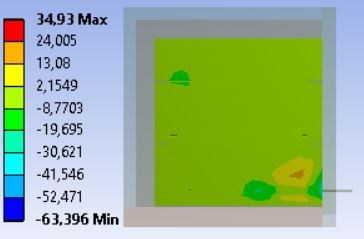
\includegraphics[width=0.7\textwidth]{4-experiment-design/img/Thermal/air-sampling-with-box}
    \caption{Cross Section of the Air in the Brain at the Time to Start Sample During Ascent.}
    \label{fig:Air-in-brain-4-6}
\end{figure}

In Figure \ref{fig:test-flight-AAC-4-6} the average temperature of the pump with data from ANSYS is presented. One was simulated with no air in the Brain and the other has air with the same density as sea level. In between the vertical dotted line is when the experiment is above 15km. At 4h in the figure the experiment is launched. It can be seen that the pump should have an average temperature over 5 degrees during the flight.
\begin{figure}[H]
    \centering
    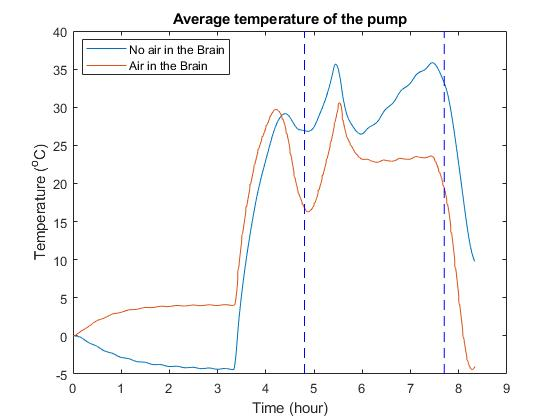
\includegraphics[width=\textwidth]{4-experiment-design/img/Thermal/pump-temperature-air-no-air.jpg}
    \caption{Temperature of the Pump Over a Simulated Flight.}
    \label{fig:test-flight-AAC-4-6}
\end{figure}

The following two figures in Figure \ref{fig:Pump-Valve-ascent-sample-4-6} were a visualization of the pump and the manifold at the time in which the AAC sampling begins during ascent. 
\begin{figure}[H]
    \centering
    \subfloat{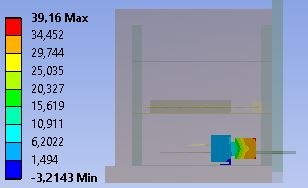
\includegraphics[width=0.46\linewidth]{4-experiment-design/img/Thermal/Pump-sampling-with-box}}
    \hifll
    \subfloat{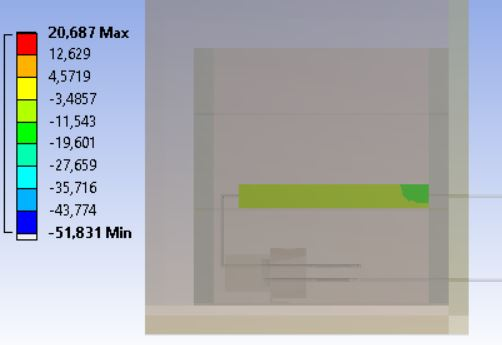
\includegraphics[width=0.45\linewidth]{4-experiment-design/img/Thermal/valve-sampling-with-box}}
    \caption{Pump and Manifold at Sampling Time During Descent With No Air in the Brain.}
    \label{fig:Pump-Valve-ascent-sample-4-6}
\end{figure}

\begin{figure}[H]
    \begin{align*}
        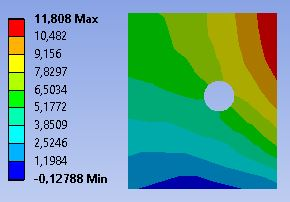
\includegraphics[width=0.5\linewidth]{appendix/img/Thermal/flushing-valve-no-air-ascent.JPG}
    \end{align*}
    \caption{Flushing Valve Prior to Sampling Commencing With No Air in the Brain.}
    \label{fig:flushing-valve-4-6}
\end{figure}

During a worst case simulation that is shown in Figure \ref{fig:Pump-Valve-ascent-sample-4-6}, the four heaters were used for 26.66 Wh in total together over the course of the simulation the figures are from. Only the pump heaters required more time if the outside were colder there was 80 Wh in the power budget table dedicated to thermal control (shown in Table \ref{tab:power-design-table}). There was therefore an incentive to keep the pump heaters on for a longer time if needed.

Based on the calculations and thermal simulations, it was concluded that the thermal designed passive and active thermal control mechanisms detailed in this section would ensure that the AAC's pump and manifold were in their operating temperature during the entire flight flight. It has been shown that the CAC has a sufficiently adequate thermal design to operate throughout the whole flight.

Thermal testing (Test 5, section \ref{Test-5}) showed that the heaters and the subsequent internal temperature responded as expected from simulations and work as required when heating the critical components. A full 4h test at $-50\degree{C}$ was done after the temperature sensor issue had been resolved and it concluded that the experiment would be able to operate thermal wise during the whole flight.


%\subsubsection{Passive Thermal Control}
%\label{sec:4.6.6}

% Description of the insulation applied (size, distribution, type of material, implementation, etc)
%It is in the appendix the thermal insulation applied - Erik
% How to deal with gaps?
% Heat sinks? (to spread high temperatures in hot spots)

%\subsubsection{Active Thermal Control}
%\label{sec:4.6.7}

% Description of the heaters performance (pictures, characteristics, locations, goal temperatures, when they work? for how long? etc.)